\chapter{Estrategia general y elementos estadísticos para una búsqueda de nueva física}\label{cap:statistical}
% \addcontentsline{toc}{chapter}{Elementos estadísticos para la búsqueda de nueva física}
\chaptermark{Estrategia general y elementos estadísticos para una búsqueda de nueva física}

% \section{Estrategia general}\label{sec:statistical}

Una estrategia para llevar a cabo una búsqueda general de nueva física, consiste a grandes rasgos en realizar un experimento de conteo de eventos con características asociadas al modelo de estudio, y su comparación con las predicciones que el Modelo Estándar hace de eventos con las mismas características. En caso de que haya un <<buen acuerdo>> entre las predicciones del SM y los datos observados, es posible afirmar que bajo las condiciones del experimento no hay evidencia de nuevos procesos físicos y que las predicciones del SM son correctas. 
Por otro lado, si se observa una discrepancia significativa (o <<exceso>>) entre las predicciones del SM y
los datos observados, se puede afirmar que el SM tiene una carencia en sus predicciones y que se podría estar en presencia de un nuevo fenómeno físico. Los criterios para definir <<buen acuerdo>> y <<exceso>> requieren evaluaciones estadísticas rigurosas que se explican en el presente Capítulo. 

\section{Regiones y modelo probabilístico}

En el contexto de esta Tesis se denomina <<señal>> a los procesos del modelo teórico que motivan dicha búsqueda, y <<fondo>> a las predicciones del SM. Para poder identificar los eventos de señal es necesario conocer las características del mismo, y luego así, discriminarlos de otros procesos físicos presentes en el experimento. Se utilizan simulaciones de Monte Carlo para modelar la señal, reconstruyendo los observables cinemáticos que caracterizan a los eventos. Aplicando diferentes cortes en esas variables se puede favorecer ciertos procesos y desfavorecer otros, y el conjunto de dichos cortes define una <<región>> en el espacio de observables. Las regiones donde la señal abunda con respecto al fondo, y por ende, donde se esperaría observar un exceso significativo en los datos, se denominan \textbf{Regiones de Señal (SR)}.

En este tipo de experimentos es fundamental un correcto modelado de los procesos de fondo,  para los cuales existen diferentes técnica. Pueden ser basadas exclusivamente en datos, exclusivamente en simulaciones de Monte Carlo, o basadas en simulaciones y  luego corregidas con los datos. La corrección de las simulaciones con datos, se debe a que las mismas en general son validadas en regiones asociadas al proceso que modelan (SM por ejemplo), y como en este caso es necesario utilizarlas en regiones de señal, probablemente alejadas o más extremas de donde se validó, es esperable que esas predicciones en esas regiones no sean del todo correctas. Para ello se definen \textbf{Regiones de Control (CR)} donde abundan eventos de algún proceso de fondo de interés, dedicadas a normalizar las simulaciones de ese proceso en particular a los datos observados en la misma, y luego poder extrapolar dicha normalización a las SRs.

Finalmente se definen \textbf{Regiones de Validación (VR)} que justamente se utilizan para validar la estimación de los fondos anteriormente mencionados, junto con la técnica de normalización y extrapolación de las CRs. Es importante destacar que el diseño de todas las regiones se realiza sin utilizar en ningún momento los datos en las SRs, lo que se denomina \textit{blinding}, para evitar así todo tipo de sesgo en el resultado del experimento. Por este motivo, como las CRs y VRs hacen uso de los datos, el diseño de las mismas debe ser ortogonal a las SRs, de tal forma que ningún dato de las SRs sea observado. A su vez, se busca que las CRs y VRs estén libres de contaminación de señal, ya que en caso de estar observándose dicha señal en los datos, la normalización y validación estaría sesgada.
Una vez que se tiene confianza en la estimación de los fondos mediante su validación en las distintas VRs, se procede a observar los datos en las SRs (\textit{unblinding}).

Complementario a las regiones del análisis, se define el método estadístico que evalúa los resultados obtenidos. El concepto central en cualquier conclusión estadística es el modelo probabilístico, el cual asigna una probabilidad a cada resultado posible del mismo. Un ejemplo muy utilizado en física de partículas, es el \textbf{Modelo de Poisson}, que describe el resultado de un experimento de conteo. Su distribución es de la forma:

\begin{equation}
	\text{Pois}(N|\mu) = \frac{\mu^{N}e^{-\mu}}{N!}
\end{equation}

\noindent
que define la probabilidad de observar $N$ veces cierto proceso aleatorio, medido en un intervalo fijo de tiempo, donde $\mu$ es el número medio de eventos esperado. La distribución de Poisson es utilizada para describir múltiples fenómenos, como decaimientos radiactivos o cualquier experimento de partículas que conste de contar eventos en un intervalo de tiempo. Es importante mencionar que las probabilidades obtenidas en esta distribución dependen estrictamente del modelo asumido como hipótesis, en este caso representado por el número medio de eventos esperados ($\mu$). De tal forma, que la probabilidad de obtener dicho número observado de eventos en el experimento, va a depender del modelo a estudiar, los cuales por ejemplo pueden ser un modelo que sólo espera fondo, o un modelo que considera la composición de fondo y señal. 

Se define adicionalmente al \textbf{\textit{Likelihood}}, como la probabilidad de ocurrencia de los datos observados ($n$) bajo la hipótesis bajo estudio, y en el caso más simple toma la forma de la distribución de Poisson:

\begin{equation}
	\mathcal{L}(n|\mu) = \text{Pois}(N=n|\mu) 
\end{equation}

\section{Likelihood máximo}

En el marco de esta Tesis se emplearon un conjunto de regiones de señal, las cuales pueden ser consideradas como experimentos de conteo independientes con distribuciones de Poisson, cuyas predicciones se obtienen a partir de simulaciones o técnicas basadas en datos. 
Es posible a su vez, realizar la búsqueda empleando distribuciones en alguna variable, las cuales requieren construir el modelo probabilístico que permita realizar predicciones de la misma. Si bien muchas distribuciones pueden ser derivadas de la teoría analíticamente, en general se utilizan simulaciones para generarlas. Esas simulaciones se describen mediante histogramas de la variable observada, y cada clase puede ser considerada como un experimento de conteo independiente (o región de señal) con una distribución de Poisson. 
Para ambos métodos el likelihood se escribe como el producto de las probabilidades de cada experimento:


\begin{equation}
	\mathcal{L}(\textbf{n}=(n_1,n_2,...)|\mu) = \prod_{i\in \text{SRs}} \text{Pois}(N=n_i|\mu) 
\end{equation}


\noindent donde $n_i$ es el número de eventos observados en cada SR. 
El likelihood puede ser utilizado adicionalmente para estimar parámetros de la teoría que estamos estudiando. Por ejemplo, si nuestro modelo está caracterizado por un conjunto de parámetros $\bm{\theta}$, y asumimos que el mismo es verdadero, se esperaría que la probabilidad de observar dichos datos para ese modelo sea máxima cuando los parámetros $\bm{\theta}$ sean lo más próximo a los valores reales del modelo. El \textbf{Estimador de Likelihood Máximo} (MLE, $\hat{\bm{\theta}}$) de un dado parámetro $\bm{\theta}$, son aquellos valores del mismo que maximizan la función likelihood. En general, para facilitar a los algoritmos computacionales de maximización, se busca en realidad el mínimo de menos el logaritmo del likelihood (LLH):

\begin{equation}
	-\ln{\mathcal{L}(\bm{\theta}}) = - \sum_{i\in \text{SRs}}\ln{\text{Pois}(n_i|\bm{\theta})}
\end{equation}

Los estimadores tienen un sesgo proporcional a la inversa del número de mediciones independientes, que en este caso es el número de regiones de señal. Cuando se tiende el número de mediciones a infinito el mismo se vuelve consistente, por lo que el valor estimado de cada parámetro converge al valor verdadero ($\bm{\theta}_0$). En dicho límite, el valor esperado del estimador coincide con $\bm{\theta}_0$ (no sesgado), y adquiere su menor varianza (eficiente).



\section{Contrastación de hipótesis}

Como se menciono anteriormente la búsqueda está caracterizada por el conjunto de parámetros del modelo empleado, que se engloban en lo que se denomina <<hipótesis>>. Con el objetivo de descubrir procesos de nueva señal, se define la \textbf{Hipótesis Nula} ($H_0$), la cual se asume como verdadera y va a estar sujeta a prueba, evaluándola contra la \textbf{Hipótesis Alternativa} ($H_1$). En el contexto de esta búsqueda, la hipótesis nula asume que no hay eventos de señal y que todo lo observado debería ser fondo, en lo que se denomina hipótesis de <<solo fondo>>. A diferencia de la alternativa, que sí predice eventos de señal, denominada hipótesis de <<señal+fondo>>. Si los resultados observados en el experimento difieren de los esperados bajo la hipótesis nula, es posible rechazar a la misma, y estar en presencia de un descubrimiento. Caso contrario de no poder rechazarla, es posible poner límites al modelo, donde los roles de las hipótesis se invierten, y ahora la hipótesis nula incluye a la señal y la alternativa solo al fondo.

Las hipótesis pueden estar completamente determinadas o estar caracterizadas por distintos parámetros, y las mismas definen a las funciones de densidad de probabilidad (PDFs\footnote{No confundir con las Funciones de Distribución Partónica, definidas en la Sección \ref{sec:qcd_pp}}) de los distintos observables. Para poder discriminar una hipótesis de otra, se define un estadístico de prueba que es una función de los observables, $t(\textbf{n})$. El mismo tendrá asociada una PDF dependiendo de la hipótesis empleada ($g(t|H)$), que al aplicarle un corte en un dado valor ($t_c$), define una región critica en el espacio de observables. Si el valor de $t$ evaluado en los datos observados ($t_{\text{obs}}$) se encuentra dentro de esa región, la hipótesis nula es rechazada. La Figura \ref{fig:nullh} muestra un esquema de lo anteriormente mencionado, en la que se puede observar la región pintada de azul ($\alpha$), denominada \textbf{Error de Tipo I}, que representa la probabilidad de rechazar $H_0$ siendo esta es verdadera. En cambio, el área roja ($\beta$), denominada \textbf{Error de Tipo II}, representa la probabilidad de aceptar $H_0$ siendo esta falsa. En un caso ideal, el estadístico de prueba obtendría los valores más pequeños posibles para $\alpha$ y $\beta$.

\begin{figure}
  \centering
  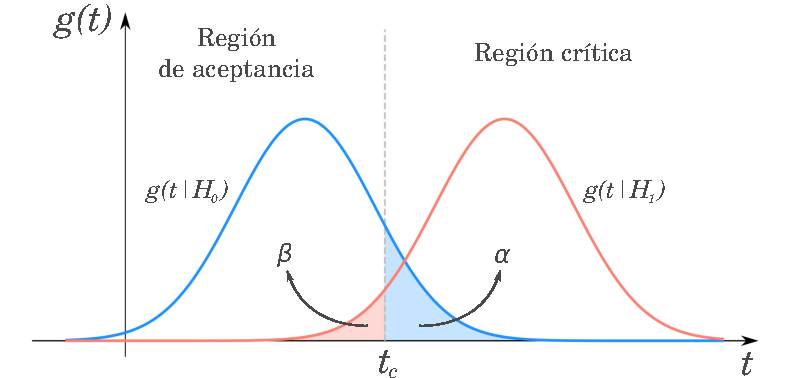
\includegraphics[width=0.8\textwidth]{images/statistics/hypo_test.pdf}
  \caption{Distribución del estadístico de prueba bajo la hipótesis nula $H_0$ (azul) y la alternativa $H_1$ (roja). El corte en $t_c$ define a la región crítica y de aceptancia. El área azul ($\alpha$) se denomina Error de Tipo I, y representa la probabilidad de rechazar $H_0$ siendo esta es verdadera. El área roja ($\beta$) se denomina Error de Tipo II, y representa la probabilidad de aceptar $H_0$ siendo esta falsa.}
  \label{fig:nullh}
\end{figure}


Alternativamente, se puede cuantizar el acuerdo entre el resultado de dicha búsqueda y una hipótesis dada, calculando el \textbf{\textit{p-value}}. El mismo se define como la probabilidad bajo dicha hipótesis, de obtener un resultado igual o menos incompatible con las predicciones de la hipótesis:

\begin{equation}
	p_H = \int_{t_{H,obs}}^{\infty} g(t|H)dt
\end{equation}

Un p-value chico implica una evidencia importante en contra de dicha hipótesis, y la misma se excluye si el p-value observado es menor a un cierto valor previamente definido.  Alternativamente se puede convertir el p-value en la significancia equivalente, $Z$. La misma se define como el número de desviaciones estándar ($\sigma$) que se debe encontrar por encima de su media, una variable con distribución Gaussiana para tener una probabilidad superior igual al p-value:

\begin{equation}
	Z=\Phi^{-1}(1-p)
	\label{ec:sign}
\end{equation}

\noindent
donde $\Phi^{-1}$ es la inversa de la cumulativa (cuantil) de la distribución Gaussiana. 


\section{Estadísticos de prueba}

% refrasear pues sacado de fran!!! Done!

El lema de Neyman-Pearson \cite{10.2307/91247} establece que el estadístico de prueba con mayor poder en la contrastación de hipótesis de <<solo fondo>> frente a hipótesis de <<señal+fondo>> (y viceversa), es el cociente de likelihoods:


\begin{equation}
	t(\textbf{n}) = \frac{\mathcal{L}(\textbf{n}|H_1)}{\mathcal{L}(\textbf{n}|H_0)}
\end{equation}

En este caso la mejor región crítica son aquellos \textbf{n} que satisfacen $t(\textbf{n})>c_\alpha$, donde $c_\alpha$ es una constante que se ajusta para que el tamaño de dicha muestra sea $\alpha$.

% El procedimiento común entonces para establecer un descubrimiento en física de partículas, se basa en un experimento frecuentista de significancia, empleando el cociente de likelihoods como estadístico de prueba. Como se mencionó anteriormente, los modelos bajo estudio están caracterizados por un conjunto de parámetros. De dichos parámetros se separan aquellos de interés ($\mu$), de aquellos que a priori no se conoce su valor y deben ser ajustados a los datos, denominados \textit{nuisance} ($\bm{\theta}$). 
El procedimiento común entonces para establecer un descubrimiento en física de partículas, se basa en un experimento frecuentista de significancia, empleando el cociente de likelihoods como estadístico de prueba. Como se mencionó anteriormente, los modelos bajo estudio están caracterizados por un conjunto de parámetros, entre los que se encuentran los <<parámetros de interés>> ($\mu$) y los <<parámetros \textit{nuisance}>> ($\bm{\theta}$). 
En el contexto de una búsqueda de nueva física, el parámetro $\mu$ representa la intensidad de la señal, de tal forma que la hipótesis de <<solo fondo>> corresponde a $\mu = 0$, y la hipótesis de <<señal+fondo>> a $\mu = 1$. En cada región del análisis uno esperaría tener un una media de eventos dada por: $\langle n_i \rangle = \mu s_i + b_i$, donde $s_i$ ($b_i$) es el número esperado de eventos de señal (fondo) en la región $i$. Por otro lado, los parámetros nuisance representan las incertezas sistemáticas, provenientes de defectos en el modelado del detector o de la teoría, que en un caso ideal se esperarían que fuesen despreciables. Para acercarse lo máximo posible a este escenario, se incluye a los mismos como parámetros a ajustar, con la consecuencia de reducir la sensibilidad del experimento.

En el caso donde hay un único parámetro de interés $\mu$, y el resto de parámetros son nuisance $\bm{\theta}$, es conveniente definir el \textit{Profile Likelihood Ratio} (PLR) \cite{Cowan:2010js}:

\begin{equation}
	\lambda(\mu)=\frac{\mathcal{L}(\mu, \doublehat{\bm{\theta}})}{\mathcal{L}(\hat{\mu}, \hat{\bm{\theta}})}
	\label{ec:plr}
\end{equation}

\noindent
donde en el denominador, los valores $\hat{\mu}$ y $\hat{\bm{\theta}}$ son los MLE de dichos parámetros. De la misma forma en el numerador, los
parámetros $\doublehat{\bm{\theta}}$ son los valores que maximizan la función likelihood, pero para un valor fijo de $\mu$. Este proceso de elegir valores específicos de los parámetros nuisance para un valor dado de $\mu$, se lo conoce como \textit{profiling}. El PLR depende explícitamente de $\mu$, pero es independiente de los parámetros nuisance que han sido <<eliminados>>
vía el profiling. La presencia de los parámetros nuisance, que son ajustados a los datos, ensanchan la función likelihood como función de $\mu$, respecto a la distribución que tendría si sus valores estuvieran fijos. De cierta forma, reflejan una pérdida de información sobre $\mu$ debido a estos parámetros desconocidos.

\section{Descubrimiento}

De la definición de $\lambda(\mu)$ se puede observar que la misma puede tomar valores solamente entre 0 y 1, donde 1 implica un buen acuerdo entre los datos y el valor hipotetizado de $\mu$. De forma equivalente es conveniente usar el estadístico de prueba:

\begin{equation}
	t_{\mu} = -2\ln{\lambda(\mu)}
\end{equation}

\noindent
donde ahora valores grandes de $t_{\mu}$ implica una gran incompatibilidad entre datos y $\mu$.

% \solved{El paper de Cowan define estadísticos de prueba alternativos, pero no sé si son los que se usan con HF. Pongo esos pero capaz no van, y lo que sigue a continuación está de más.} SI son

En muchos análisis, la contribución del proceso de señal al valor medio de eventos, se asume como no negativo, lo que implica que cualquier estimador de 
$\mu$ debería ser no negativo. Aún si no fuese así el caso, es conveniente definir un estimador efectivo $\hat{\mu}$ que maximice el likelihood y que tenga la posibilidad de tomar valores negativos (siempre y cuando los valores medios de Poisson, $\mu s_i + b_i$, sean no negativos). Esto va a permitir más adelante modelar a $\hat{\mu}$ como una variable con distribución Gaussiana. 

Para un modelo con $\mu\ge0$, si se encuentra que su estimador es negativo ($\hat{\mu}<0$), entonces el mejor nivel de acuerdo entre datos y cualquier valor físico de $\mu$ va a ser cuando $\mu=0$. Por lo que se puede redefinir al PLR ($\tilde{\lambda}$) para generar un test estadístico alternativo que tenga en cuenta esto:

\begin{equation}
	\tilde{t}_{\mu}=-2\ln{\tilde{\lambda}(\mu)}=
	\begin{cases}
		-2\ln{\frac{\mathcal{L}(\mu, \doublehattwo{\bm{\theta}}(\mu))}{\rule{0pt}{0.49em} \mathcal{L}(0, \doublehattwo{\bm{\theta}}(0))}} & \hat{\mu}<0 \\
		-2\ln{\frac{\mathcal{L}(\mu, \doublehattwo{\bm{\theta}}(\mu))}{\rule{0pt}{0.49em} \mathcal{L}(\hat{\mu}, \hat{\bm{\theta}})}} & \hat{\mu}\ge0 
	\end{cases}
\end{equation}


Un caso especial de este estadístico de prueba es cuando se analiza la hipótesis de <<solo fondo>> ($\mu=0$), ya que el rechazo de la misma puede llevar al descubrimiento de nueva señal:

\begin{equation}
	q_{0}=
	\begin{cases}
		0 & \hat{\mu}<0 \\
		-2\ln{\lambda(0)} & \hat{\mu}\ge0\\
	\end{cases}
	\label{eq:st_q0}
\end{equation}

Si los datos observados resultan menores a las predicciones del fondo, se tiene $\hat{\mu}<0$. Esto podría significar una evidencia en contra de la hipótesis de <<solo fondo>>, pero en realidad no muestra que los datos estén compuestos de eventos de señal. Con esta definición entonces, la posibilidad de descartar la hipótesis de <<solo fondo>> ocurre solo cuando $\hat{\mu}\ge0$, y en caso contrario $q_{0}=0$. El p-value para este estadístico de prueba queda entonces:

\begin{equation}
	p_0 = \int_{q_{0, \text{obs}}}^{\infty} f(q_0|0)dq_0
	\label{ec:pvalue_0}
\end{equation}

La comunidad de física de partículas tiende a definir un rechazo de hipótesis de <<solo fondo>> con una significancia superior a los $5\sigma$ ($p=2.87 \cdot 10^{-7}$) como un nivel apropiado para definir un descubrimiento. Para excluir hipótesis de señal se define en cambio a partir de $1.64$ sigmas ($p=0.05$). Cabe destacar que el rechazar la hipótesis de solo fondo es solo parte del proceso de descubrimiento de un nuevo fenómeno. La certeza de que un nuevo proceso está presente va a depender en general de otros factores, como la plausibilidad de una nueva hipótesis de señal, y el grado al cual la misma describe a los datos observados.

\section{Límites superiores de exclusión}

Cuando el p-value obtenido es mayor al límite definido para un descubrimiento, no es posible rechazar la hipótesis de <<solo fondo>>, y en ese caso se desea establecer límites sobre el modelo caracterizado. Para ello se busca rechazar la hipótesis <<señal+fondo>>, y encontrar el valor de $\mu$ para el cual no es más posible seguir haciendo ese rechazo (límite superior). Se define entonces un nuevo estadístico de prueba, donde los roles de la hipótesis de <<solo fondo>> de <<señal+fondo>> son intercambiados:


\begin{equation}
	\tilde{q}_{\mu}=
	\begin{cases}
		-2\ln{\tilde{\lambda}(\mu)} & \hat{\mu}\le\mu \\
		0 & \hat{\mu}>\mu \\
	\end{cases}=
	\begin{cases}
		-2\ln{\frac{\mathcal{L}(\mu, \doublehattwo{\bm{\theta}}(\mu))}{\rule{0pt}{0.49em} \mathcal{L}(0, \doublehattwo{\bm{\theta}}(0))}} & \hat{\mu}<0 \\
		-2\ln{\frac{\mathcal{L}(\mu, \doublehattwo{\bm{\theta}}(\mu))}{\rule{0pt}{0.49em} \mathcal{L}(\hat{\mu}, \hat{\bm{\theta}})}} & 0\le\hat{\mu}\le \mu \\
		0 & \hat{\mu}>\mu \\
	\end{cases}
	\label{ec:st_qmu}
\end{equation}

% sacado de fran

% \solved{Este párrafo no lo entiendo bien} ya esta

La razón para poner $\tilde{q}_{\mu} = 0$ para $\hat{\mu}>\mu$ es que cuando se establece un límite superior, el hecho de que $\hat{\mu}>\mu$ representa menos compatibilidad con $\mu$ que los datos obtenidos, y por lo tanto no se considera parte de la región de rechazo de la contrastación. Cabe destacar que el $\tilde{q}_0$ anteriormente definido, no es un caso particular de este estadístico de prueba, ya que $q_0$ es cero si los datos fluctúan hacia abajo ($\hat{\mu}<0$), pero $\tilde{q}_{\mu}$ es cero si los datos fluctúan hacia arriba ($\hat{\mu}>\mu$).

Con este estadístico de prueba se busca encontrar el valor de $\mu$ para el cual deja de ser posible el rechazo de la hipótesis <<señal+fondo>> (o viceversa, hasta que valor de $\mu$ es posible un rechazo de la hipótesis). Para ello se definen el nivel de confianza \cite{Read:2002hq}:

\begin{equation}
	\text{CL}_{s} = \frac{p_{\mu}}{1-p_{b}} \equiv \frac{\text{CL}_{s+b}}{\text{CL}_{b}}
\end{equation}


\noindent 
donde

\begin{equation}
	p_{\mu} = \int_{q_{\mu, \text{obs}}}^{\infty} f(q_\mu|\mu)dq_\mu \equiv \text{CL}_{s+b} \quad\quad\quad \text{y} \quad\quad\quad 1-p_b = \int_{q_{\mu, obs}}^{\infty} f(q_\mu|0)dq_\mu \equiv \text{CL}_{b}
	\label{ec:pvalue_mu}
\end{equation}

\noindent
siendo $f(q_\mu|\mu)$ la PDF del estadístico de prueba $q_\mu$, y $f(q_\mu|0)$ la PDF bajo la hipótesis de <<solo fondo>>. Cuanto más bajo es el $\text{CL}_{s}$, menos compatibilidad entre los datos y la hipótesis de <<señal+fondo>>. Se define por convención al límite superior ($\mu_{\text{up}}$) como aquel $\mu$ que tiene un $\text{CL}_{s}=5\%$, y se rechazan entonces lo modelos con $\mu$ menores a $\mu_{\text{up}}$. La ventaja de usar $\text{CL}_{s}$ en vez de directamente $\text{CL}_{s+b}$, radica en que este último puede excluir hipótesis de <<señal+fondo>> cuando es semejante a la de <<solo fondo>>, y el número de eventos observados es mucho menor que el de fondo. Esto no es deseado, ya que en la práctica no se pretende excluir hipótesis de las cuales no se tiene sensibilidad alguna. 




\section{Aproximación de las distribuciones de los estadísticos de prueba}\label{sec:aprox_test}

Para hallar el p-value de una hipótesis es necesaria la función densidad de probabilidad del estadístico de prueba. Por ejemplo, para rechazar la hipótesis nula se calcula el p-value, que depende de $f(q_{0}|0)$ como muestra la Ecuación \ref{ec:pvalue_0}. Para poner límites superiores al modelo se necesita $f(q_{\mu}|\mu)$ y $f(q_{\mu}|0)$, como se ve en la Ecuación \ref{ec:pvalue_mu}. Inclusive se requiere de $f(q_{\mu}|\mu')$ con $\mu\neq\mu'$, para hallar la significancia esperada, empleada en la evaluación a priori de la sensibilidad del análisis (Sección \ref{sec:exp_sig}). En un principio dichas PDFs son desconocidas analíticamente, pero es posible obtenerlas empleando métodos alternativos.

Considerando al PLR de la Ecuación \ref{ec:plr}, determinado por el parámetro $\mu$, que puede ser cero (descubrimiento), o no (límites superiores), y suponiendo que los datos se distribuyen de acuerdo a un parámetro $\mu'$. La distribución $f(q_{\mu}|\mu')$ se puede aproximar utilizando el teorema de Wald \cite{10.2307/1990256}, que muestra que para el caso de un solo parámetro de interés:

\begin{equation}
	-2\ln{\lambda(\mu)}=\frac{(\mu-\hat{\mu})^{2}}{\sigma^{2}}+\mathcal{O}(1/\sqrt{N})
\end{equation}

\noindent
donde $\mu$ sigue una distribución Gaussiana con una media $\mu'$ y una desviación estándar $\sigma$, y $N$ representa el tamaño de la muestra. 
% Si despreciamos el término $\mathcal{O}(1/\sqrt{N})$ se puede mostrar que el estadístico de prueba $t_{\mu}$ sigue una distribución de $\chi^{2}$ no central con un grado de libertad.
En el límite asintótico se puede mostrar que el estadístico de prueba $t_{\mu}$ sigue una distribución de $\chi^{2}$ no central con un grado de libertad, y en ese caso el estadístico de prueba para descubrimiento ($q_{0}$) de la Ecuación \ref{eq:st_q0} puede aproximarse como:

\begin{equation}
	q_{0}=
	\begin{cases}
		0 & \hat{\mu}<0 \\
		\hat{\mu}^{2}/\sigma^{2} & \hat{\mu}\ge 0 \\
	\end{cases}
\end{equation}

De la misma forma, a su respectivo p-value se lo puede aproximar como $p_{0}=1-\Phi(\sqrt{q_{0}})$ y a la significancia equivalente como $Z_{0}=\sqrt{q_{0}}$. La misma aproximación vale para el estadístico de prueba para límites superiores ($\tilde{q}_{\mu}$) de la Ecuación \ref{ec:st_qmu}, cuya expresión se describe en la Referencia \cite{Cowan:2010js}.

Cuando la estadística es reducida ($\mathcal{O}(10)$), se abandona el régimen asintótico, y las aproximaciones anteriores dejan de tener validez. En ese caso el estadístico de prueba se obtiene a partir de lo que se denominan \textit{toys} o <<psuedo-experimentos>> \cite{Baak:2014wma}. Para ello se varían los parámetros $\mu_\text{sig}$ y $\bm{\theta}^0$, generando una estadística suficiente para tener una estimación conservadora del p-value, y por ejemplo, si se obtiene un $\text{CL}_{s}>5\%$ para alguna de esas variaciones, no es posible excluir a la hipótesis empleada. Este método puede resultar poco práctico, sobre todo cuando hay un gran número de sistemáticos, y se puede entonces realizar una estimación de los parámetros $\bm{\theta}^0$ que maximizan el p-value. Para ello inicialmente se ajustan dichos parámetros a los datos observados y basándose en un dado valor de $\mu_\text{sig}$. Los valores obtenidos para $\bm{\theta}^0$ mediante este ajuste son luego empleados para las siguientes iteraciones que permiten calcular el p-value. El hecho de emplear datos al realizar los toys, genera una dependencia residual en el cálculo de algunos límites, obtenidos solamente a partir de las estimaciones de fondo esperadas.
 



% \solved{Debería explicar Asimov?} nope

 
% Estas aproximaciones permiten conocer las distribuciones muéstrales y calcular valores-p y significancias en el caso de un gran número de datos, de una forma simple y computacionalmente poco
% costosa. A pesar de que estrictamente es válido para $N\to\infty$, esta aproximación es suficientemente
% precisa para un número de eventos de fondo $\sim \mathcal{O}(10)$.
% Para muestras de datos muy pequeñas, o en casos donde la precisión es importante, siempre pueden
% validarse estas aproximaciones utilizando la generación Monte Carlo. Para esto es necesario utilizar
% simulaciones Monte Carlo para generar lo que se denomina `pseudo-experimentos'. El procedimiento
% consiste en generar el conjunto de observables x utilizando la pdf $f(x|H)$ y calcular el valor del
% estadístico de prueba $t(x)$ para cada conjunto. Este proceso se repite hasta acumular suficiente
% estadística en la distribución muestral del estadístico $g(t|H)$.

\section{Significancia esperada}\label{sec:exp_sig}

El diseño de las regiones de señal para el análisis es un proceso denominado <<optimización>>, que define el conjunto de cortes óptimo para discriminar el fondo de la señal. Tal discriminación es cuantizada mediante la significancia de la Ecuación \ref{ec:sign}, la cual a priori es desconocida. Para estimar el valor de significancia ($Z$) que uno esperaría tener en un dado experimento, con un número de eventos igual a la suma de las estimaciones de fondo y señal ($n=s+b$), se puede emplear la significancia esperada, que se define como la mediana de $Z$. Como el p-value y $Z$ tienen una relación lineal y monotónica \cite{Cowan:2010js}, la mediana de $Z$ se puede obtener a partir de la mediana del p-value.


Por ejemplo, si tenemos una variable $n$ que sigue una distribución de Poisson y tiene media $s+b$, si la media es lo suficientemente grande, es posible aproximar a la misma mediante una distribución Gaussiana, con media $s+b$ y desviación estándar $\sqrt{s+b}$. El p-value para la hipótesis de <<solo fondo>> ($s=0$) dada una observación $n$ es:

\begin{equation}
	p = 1 - \Phi\left( \frac{n-\mu}{\sigma} \right) = 1 - \Phi\left( \frac{n-b}{\sqrt{b}} \right)
\end{equation}

Lo que permite obtener la significancia para descubrimiento:

\begin{equation}
	Z = \frac{n-b}{\sqrt{b}}
\end{equation}

La media de $Z$ coincide con la mediana, y como la media de $n$ es $s+b$, se obtiene:

\begin{equation}
	\text{med}[Z|s] = \frac{s}{\sqrt{b}}
\end{equation}

Esta magnitud fue históricamente empleada en física de partículas para la estimación de la significancia esperada. La misma se puede interpretar como la fracción de eventos esperados de señal, con respecto a la incerteza estadística del número esperado de eventos total, asumiendo la ausencia de señal.

Si el numero esperado de eventos de fondo $b$ es desconocido, debe ser incluido como parámetro nuisance. En ese caso $b$ puede ser ajustado libremente al número de eventos observados, y sería imposible rechazar la hipótesis de <<solo fondo>> ($s=0$), a menos que se introduzca información adicional que limite dicho parámetro. Para ello, se incluyen las regiones de control, donde no hay eventos de señal y donde la estimación del fondo en esta región puede relacionarse con la estimación en las regiones de señal. Estas regiones son incluidas aa la función likelihood como distribuciones de Poisson, de igual forma que las regiones de señal. Procediendo de forma similar que en el ejemplo anterior, empleando la hipótesis de <<solo fondo>> ($s=0$) y la aproximación mediante <<datos de Asimov>> \cite{Cowan:2010js}, se puede obtener una expresión para la significancia esperada en función de la estimación del fondo, basada en la región de control y su incertidumbre ($\sigma_b$):

\begin{equation}
	Z = \sqrt{ 2 (s+b) \ln{\left[ \frac{(s+b)(b+\sigma_b^2)}{b^2 + (s+b)\sigma_b^2} \right]} - \frac{2 b^2}{\sigma_b^2} \ln{ \left[ 1 + \frac{s \sigma_b^2}{b(b+\sigma_b^2)} \right] } }
\end{equation}

La estimación de la significancia esperada depende también del tipo de experimento que se desea realizar. En la práctica se emplea un método descripto en las Referencias \cite{Linnemann:2003vw, stat_1, ATL-PHYS-PUB-2020-025}, y que se engloba en una función del framework \texttt{ROOT} \footnote{\texttt{ROOT.RooStats.NumberCountingUtils.BinomialExpZ}}, que depende de la estimación de la señal y fondo, junto con su incertidumbre. 
% En general, para la incerteza del fondo se hace una estimación conservadora del 30\%. 

% La búsqueda comienza definiendo las regiones de señal. Las mismas están caracterizadas por un estado final (motivado por un modelo en particular) que determina los cortes preliminares de la región. Adicional a esos cortes se agregan otros que aumentan el poder discriminatorio de las regiones de señal. El proceso de definir el conjunto de SRs y los cortes más aptos de cada una se denomina optimización. Es posible definir un conjunto de SRs optimizadas para discriminar al mismo modelo pero con distintos parámetros (masas por ejemplo), pudiendo estas ser independientes entre sí u ortogonales. Esto último puede ser ventajoso dependiendo de si se está realizando la búsqueda con el objetivo de descubrir algún fenómeno, o si se quiere poner límites al modelo estudiado. Cabe mencionar que si bien se buscan las regiones con mayor poder discriminatorio, es importante evitar definirlas basándose fuertemente en las predicciones del modelo. En caso de realizar una búsqueda muy dependiente del modelo y de no observar un exceso, se estarían poniedo límites a un modelo muy particular resultando poco útil para la comunidad científica. En por eso que el proceso de optimización, si bien está motivado por un estado final determinado por el modelo, termina siendo un compromiso entre un buen poder discriminatorio sin perder la idependencia al mismo. Una forma de garantizar esa independiencia es utilizar cortes un poco más relajados y pedir un número mínimo de eventos de señal y fondo.




% \section{Ajuste de solo fondo}

% Key ingredients of the fitting procedure are the ratios of expected event counts, called transfer
% factors, or TFs, of each normalized background process between each SR and each CR. The TFs
% allow the observations in the CRs to be converted into background estimates in the SRs, using:

% \begin{equation}
%     N^{(SR)}_{p}(est.) = N^{(SR)}_{p}(raw) \times \frac{N^{(CR)}_{p}(obs.)}{N^{(CR)}_{p}(est.)} = \mu_{p} \times N^{(SR)}_{p}(raw)
% \end{equation}

% where Np(SR,est.) is the SR background estimate for each simulated physics processes p considered
% in the analysis, Np(CR,obs.) is the observed number of data events in the CR for the process, and
% MCp(SR,raw) and MCp(CR,raw) are raw and unnormalized estimates of the contributions from
% the process to the SR and CR respectively, as obtained from MC simulation. An important feature of using TFs is that systematic uncertainties on the predicted background
% processes can be canceled in the extrapolation; a virtue of using the ratio of MC estimates. The total uncertainty on the number of background events in the SR is then a combination of the
% statistical uncertainties in the CR(s) and the residual systematic uncertainties of the extrapolation.
% For this reason, CRs are often defined by somewhat looser cuts than the SR, in order to increase
% CR data event statistics without significantly increasing residual uncertainties in the TFs, which in
% turn reduces the extrapolation uncertainties to the SR


\section{Modelo estadístico y flujo de búsqueda}

La función de likelihood empleada para esta tesis se escribe como:

% \solved{Traté de que incluya la mayor información posible en una sola expresión, inclusive el ajuste solo fondo. Como en algunos ajustes se incluye el muSig en las CR (es cierto?), me pareció que podía poner a todas las regiones en una misma productoria (en el paper separan SR de CR porque a las CR no les incluye señal). También puse explícito el TF para los fondos que corresponda.} solved

\begin{equation}
	\begin{split}
	& \mathcal{L} (\textbf{n} | \mu_\text{sig}, \bm{\mu}_{\text{bkg}}, \textbf{s}, \textbf{b}, \bm{\theta}) = P_\text{SR} \times P_\text{CR} \times  C_\text{syst} (\bm{\theta}^0, \bm{\theta}) \\
	& = \prod_{i \in \text{SR}} \frac{(\mu_\text{sig} s_i + \bm{\mu}_{\text{bkg}} \cdot \textbf{b}_i)^{n_i}}{n_i!} \prod_{j \in \text{CR}} \frac{(\mu_\text{sig} s_j + \bm{\mu}_{\text{bkg}} \cdot \textbf{b}_j)^{n_j}}{n_j!} \prod_{k \in S} G(\theta_k^0 - \theta_k) \\
	\end{split}
	\label{eq:analysis_lh}
\end{equation}


La misma se compone de la distribución de los datos observados en cada SR y CR, y un factor adicional que engloba las incertezas sistemáticas. En una dada región $i$, los datos observados ($n_i$) obedecen la distribución de Poisson con media $\mu_\text{sig} s_i + \bm{\mu}_{\text{bkg}} \cdot \textbf{b}_i$, donde $\mu_\text{sig}$ es la intensidad de señal, $s_i$ es la estimación de señal, $\textbf{b}_i = (b_i^{(1)}, b_i^{(2)}, ...)$ es la estimación de cada fondo, y $\bm{\mu}_{\text{bkg}} = (\mu^{(1)}, \mu^{(2)}, ...)$ son los factores de normalización de cada fondo (cuyo uso se explica más adelante). Las incertezas sistemáticas ($S$) son parametrizadas mediante $\bm{\theta}$, y son incluidas usando la PDF $C_\text{syst} (\bm{\theta}^0, \bm{\theta})$, donde $\bm{\theta}^0$ (generalmente fijadas a 0) son los valores centrales de las medidas auxiliares a partir de los cuales el parámetro $\bm{\theta}$ puede fluctuar al realizar un ajuste. Las variaciones de estos parámetros nuisance tiene un impacto directo en las estimaciones de los fondos y señal ($\textbf{b}_i$ y $s_i$). Para parámetros nuisance independientes, esta PDF es simplemente el producto de cada incerteza, la cual corresponde con una Gaussiana con media $\theta_i^0 - \theta_i$. Los términos para las SRs y CRs fueron separados explícitamente debido a que pueden ser modificados de acuerdo al tipo de ajuste que se realice. 

El estadístico de prueba empleado es el PLR descripto en la Ecuación \ref{ec:plr} a partir del likelihood de la Ecuación \ref{eq:analysis_lh}, y modificado para la evaluación del descubrimiento (Ecuación \ref{eq:st_q0}) o para los límites de exclusión (Ecuación \ref{ec:st_qmu}).

La búsqueda comienza con el diseño de las SRs, a partir de la estimación de los procesos de señal y fondo, buscando maximizar la significancia esperada descripta en la Sección \ref{sec:exp_sig}. Luego se diseñan las CRs, con el objetivo de normalizar los fondos de MC principales a los datos observados, realizando lo que se denomina el \textbf{Ajuste de solo fondo (blinded)}. Para ello se omite en el likelihood el término de las SRs y se fija $\mu_\text{sig}=0$. Con dicho ajuste es obtienen los \textbf{factores de transferencia} ($\bm{\mu}_b$), que se aplican a los respectivos fondos para corregir la estimación de los mismos a los datos en las CRs, y luego extrapolar dicha corrección a todas las regiones del análisis de la forma:

% \solved{Acá mes desvié un poco con la notación, corregir!} done

% \begin{equation}
%     N^{(SR)}_{p}(est.) = N^{(SR)}_{p}(raw) \times \frac{N^{(CR)}_{p}(obs.)}{N^{(CR)}_{p}(est.)} = \mu_{p} \times N^{(SR)}_{p}(raw)
% \end{equation}


\begin{equation}
	n_i^{\text{(p)}} = \frac{n_{\text{CR}}}{b_{\text{CR}}^{\text{(p)}}} \times b_i^{\text{(p)}} = \mu^{\text{(p)}} \times b_i^{\text{(p)}}
\end{equation}

Una ventaja de emplear este método, es que las incertezas sistemáticas en las predicciones de los fondos se cancelan parcialmente en dicha extrapolación. La incerteza total en el número de fondo en cada región, es una combinación de la incerteza estadística de las CRs, y el residual de las incertezas sistemáticas. Para ello se emplea en las CR cortes más relajados, con la idea de aumentar la estadística, sin incrementar las incertezas residuales, lo cual reduce la extrapolación de las incertezas a las demás regiones. La extrapolación de las incertezas sistemáticas es un proceso complejo basado en la construcción de las PDF tanto en las CRs como en las SRs y VRs, la cual se describe en detalle en las Referencias \cite{Baak:2014wma, Cranmer:1456844}. Aquellos fondos que no son normalizados en las CRs dedicadas, simplemente emplean $\mu^{\text{(p)}}=1$. El objetivo final de este ajuste realizar una estimación adecuada de los fondos en las regiones del análisis, principalmente validando dicho método en las VRs del análisis.

Una vez que se considera que el modelado de los fondos es el adecuado, se procede a observar los datos en las SRs (\textit{unblinding}), el cual permite evaluar si se está en presencia de un descubrimiento o no. Se realiza el ajuste del likelihood ahora con la hipótesis de <<solo fondo>> ($\mu_\text{sig}=0$), pero incluyendo también las SRs (\textbf{Ajuste de solo fondo (unblinded)}). El parámetro $\bm{\mu}_b$ es nuevamente ajustado (junto con los sistemáticos), el cual se espera que dé resultados semejantes al ajuste sin SRs. A su vez, en el denominador del estadístico de prueba, tanto $\bm{\mu}_b$ como $\mu_\text{sig}$ son parámetros ajustables, aunque la contribución de señal es desconocida. Para ello se emplea una señal \textit{dummy}, en donde $s_i=1$, y $\mu_\text{sig}$ representa directamente el número de eventos de señal estimado en cada SR, y en las CR directamente se asume que no hay contribución de señal ($s_i=0$). 
A partir del likelihood obtenido se calcula el estadístico de prueba para descubrimiento observado ($q_{0, obs}$), y con ello el p-value del mismo. Dicho valor permite  afirmar si la observación corresponde al descubrimiento de un nuevo fenómeno.

En caso de no poder confirmar un descubrimiento es posible imponer límites sobre el modelo estudiado, en lo que se denomina \textbf{Ajuste dependiente del modelo}. 
Se realiza entonces el ajuste del likelihood pero ahora empleando la hipótesis de <<señal+fondo>> ($\mu_\text{sig}=1$), y considerando la contribución de la señal tanto en las SRs como en las CRs, la cual se estima mediante simulaciones de MC. Luego se obtiene el estadístico de prueba para límites observado ($q_{\mu, obs}$) y se calcula el $\text{CL}_{s}$. Este ajuste se realiza para cada modelo de señal, que se generan variando algún parámetro (masa por ejemplo), el cual toma valores discretos. El límite se define como aquellos puntos de señal para los cuales se encuentra un $\text{CL}_{s}=5\%$. Generalmente ningún punto del modelo cumple exactamente esta condición y es necesaria realizar una interpolación entre los puntos más cercanos a ese valor de $\text{CL}_{s}$, permitiendo así obtener el límite en función del parámetro de forma continua. Existen dos tipos de límites, el observado y el esperado. El primero emplea en el likelihood los datos observados para calcular el $q_{\mu, obs}$, mientras que en el segundo la integral que se realiza para el $\text{CL}_{s}=5\%$, se realiza desde la mediana de la PDF de la hipótesis de <<solo fondo>>. Esto sería el equivalente a calcular una significancia esperada, pero invirtiendo los roles de la hipótesis <<solo fondo>> y <<señal+fondo>>.
El límite esperado se puede calcular inclusive antes de realizar el unblind, para evaluar la sensibilidad que se obtiene mediante las regiones de señal diseñadas.

Para ampliar la utilidad de los resultados obtenidos en el análisis, es posible a su vez establecer límites independientes del modelo, mediante lo que se denomina \textbf{Ajuste independiente del modelo}. Para ello se establecen límites superiores al número de eventos en cada SR, de forma de poder saber si algún modelo alternativo ya está excluido por el análisis actual, simplemente estimando el número de eventos de dicho modelo en las SRs. Se realiza entonces un ajuste del likelihood, donde nuevamente no se permite contaminación de señal en las CR, y donde se emplea una señal \textit{dummy} en las SRs ($s_i=1$). Como ahora también el parámetro $\mu_\text{sig}$ es ajustable, puede ocurrir que el número de eventos esperado en las SRs se modifique con respecto a las estimaciones iniciales. El estadístico de prueba queda ahora en función de $\mu_\text{sig}$, y el límite en el número de eventos se define como aquel $\mu_\text{sig}$ cuyo $\text{CL}_{s}=5\%$. Para ello se calculan los valores de $\text{CL}_{s}$ probando distintas distribuciones del estadístico de prueba, con valores de $\mu$ discretos, y buscando aquellos que se obtenga un $\text{CL}_{s}$ cercano al 5\%. Luego se realiza una nueva evaluación más refinada empleando el valor obtenido con la iteración anterior. Nuevamente se pueden obtener límites observados y esperados, de la misma forma que se realizó para lo límites dependientes del modelo.

